\documentclass[twoside,11pt]{article}

% !!!!! As a rule, use past tense to describe events that have happened. Such events include procedures that you have conducted and results that you observed. Use present tense to describe generally accepted facts. !!!!!

% Any additional packages needed should be included after jmlr2e.
% Note that jmlr2e.sty includes epsfig, amssymb, natbib and graphicx,
% and defines many common macros, such as 'proof' and 'example'.
%
% It also sets the bibliographystyle to plainnat; for more information on
% natbib citation styles, see the natbib documentation, a copy of which
% is archived at http://www.jmlr.org/format/natbib.pdf

\usepackage{jmlr2e}
\usepackage{amssymb} %maths
\usepackage{amsmath} %maths
\usepackage{multirow}
\usepackage{rotating}
\usepackage{url}

\newcommand{\dataset}{{\cal D}}
\newcommand{\fracpartial}[2]{\frac{\partial #1}{\partial  #2}}

\ShortHeadings{Location Classification on Tweets}{Erdi \c{C}all{\i}}
\firstpageno{1}

\begin{document}

\title{Location Classification on Tweets}
\author{\name Erdi \c{C}all{\i}  \email e.calli@student.ru.nl}
\maketitle
\begin{abstract}
% Previous research on Twitter user location classification is mostly focusing on multi-class prediction. Approaching at the same problem from another perspective, in some cases, it may be enough to answer if someone belongs to a location or not. In this perspective, we have compared some models for predicting tweet locations using Binary and Multi-Class Classification. We have seen that if the problem at hand is reducible to Binary Classification, it is possible to make much better predictions.

\end{abstract}


\section{Introduction}

Twitter is an online platform that lets users to share posts with their followers, limited with at most 140 characters, called as tweets. Tweets can be almost anything that we share on internet; a personal message stating our views, a link to an article, a picture and etc.. There are no boundaries except the character limit. In 2009, Twitter introduced an option to include geographic location(geolocation) information on tweets\footnote{\url{https://blog.twitter.com/2009/location-location-location}}. Since then, a lot of twitter users have been sharing their geolocation with their tweets(or geotagging their tweets). Depending on the context of the tweet, having the geolocation may be very valuable. For example a tweet about a Pizza franchise or a political campaign, if geotagged, may point to an improvement with exact location or contribute to the statistics of a specific area. Unfortunately, geolocation of a tweet is not shared by default or in other words, most of the tweets are not geotagged, unless explicitly specified. Inferring the geolocation of a tweet is what this paper is about.

To be able to infer this information, we can try to use linguistic habits shared by the people who are within the same location. As humans, our spatial cognition deals with updating and managing the knowledge about our environment. Spatial cognition changes when we move between environments, but as we stay within the boundaries of a high level environment(i.e. state, city, borough), there may be some high-level constants that doesn't change. If some of these constants are shared commonly between people, it may lead them to have similar linguistic habits, in this case, textual features in their tweets. If we group the geotagged tweets sent within a high-level location, it may be possible to extract these features, if they exist.

Using similar features, previous research tries to determine the geolocation of a tweet using multi-class classification algorithms. These methods are trying to determine the most likely geolocation for a tweet from a list(e.g. cities in a country). It is sometimes hard to do that, because we need data from all cities. Also the algorithms and the implementations become more complicated. Thus, in cases where we just want to know if someone is within a state/city/borough or not, this approach becomes unnecessarily heavy. In this research, we are simplifying this problem by using binary classification algorithms, which are trying to determine if a tweet sent within the boundaries of a location(i.e. Manhattan, NY) or not. 

Revolving around our hypothesis, the research question we're trying to answer is: "Are there textual features in tweets, that are common for people within the same location? If there are, can they help us determine if a tweet is sent within that high-level location, or not?"


\section{Related Work}

% Using text mining methods and location tags in tweets, \cite{cheng2010you} redefined this problem. \cite{cheng2010you} used only the text data and introduced a method that identifies the words with strong local geo-scope. This study achieved up to 51\% accuracy to locate users within a 100 mile radius. 

% \cite{hecht2011tweets} introduced the $CALGARI$ classifying algorithm specific to this problem, focusing on country and state prediction. They got a 72\% accuracy for classifying 4 countries and 30\% accuracy on classifying 18 states. 

% \cite{eisenstein2010latent} created a geographic topic model to make use of the textual differences in topics based on regions, they got a median distance error of 494 kms. 

% \cite{wing2011simple} tried to solve this problem using geotagged Wikipedia articles and tweet texts, focusing on predicting the geolocation. Their work has obtained a median error of 479 km's for tweets. 

% \cite{mahmud2012tweet} introduced hierarchical classification methods combined with statistical methods. They have achieved 58\%, 66\% and 78\% accuracy on city, state and timezone levels, respectively. Also their findings show that users may be able to partially hide their locations, making their tweets untraceable. Same researchers revisited the problem in \cite{mahmud2014home}, trying to classify the home location of users, achieving similar results and also introducing movement and location prediction. 

% \cite{sadilek2012finding} approached this problem introducing the friend information, constructing a friend location graph. Their study was able to achieve 77\% to 84.3\% accuracy, relative to available number of friends.

% \cite{graham2014world} studied the problems with the baselines accepted by recent studies and explained why location and language classification is not an easy problem and how some of the assumptions are incorrect, such as accepting the device location as user's location. 

\section{Method}
\subsection{Data Collection and Filtering}

Using Twitter's sample status streaming api\footnote{https://dev.twitter.com/streaming/reference/get/statuses/sample}, we have sampled the public tweets. This api samples approximately 1\% of all the public tweets around the world. To be able to find the tweets that are relevant to our task, we have applied some filters to this api. 

First of all, we have applied a filter to ignore non-geotagged tweets. The high-level location information contained within each geotag will be used as the label of a tweet. These labels will be used to train our algorithms, and they will be compared with the predicted results to see how accurate our methods are.

Also, we are not interested with tweets in different languages. Having tweets from different languages would introduce a complicated variable and make our results hard to interpret. Therefore, we choose English as our language of interest, because we assumed that English is the most common language that people tweet, thus it would yield the biggest dataset(compared to other languages). Samples from twitter contain the language information, we have used this information to filter tweets which are not English. 

Considering the language assumption, having tweets from non-English speaking countries would be unnecessary. Also, having tweets from different countries would introduce another variable. Assuming that United States would yield the biggest dataset(compared to other countries), we have limited the tweets we collected to United States.

Running the data collector for 1 month, we have collected a dataset consisting of 33112 tweets, geotagged within United States, tagged as English and each from a unique user.

Since each tweet is consisting of at most 140 characters, our dataset might not be enough to extract the textual features we're interested in. To enrich our database, we assumed that our users are not actively travelling. Therefore, we have collected past 40(at most) tweets of these users and attached them to the sampled tweet as history.

Assuming we had a dataset, big enough for the task, we examined a small sample of it. In this sample, we have seen many examples which were not composed by humans, but bots(e.g. "\textit{Police department activity on \#I95 SB at 3rd Avenue; Exit 3}"). Twitter also gives the information on which application is used to send a tweet. We have examined this information, called \textit{source}, to filter these tweets. Grouping and sorting them by the number of tweets, we were able to see which sources are most relevant for our study. Annotating the most relevant 20(e.g. \textit{Twitter for iPhone}, \textit{Facebook} and etc.) we have created the whitelist filter for tweet sources.

In our examination, we have also seen a variety of geotag names which represent the high-level locations we're interested in(e.g. \textit{Mississippi, USA}, \textit{Manhattan, NY} and etc.). When we checked the number of tweets per location, we have seen that there are 4898 unique locations in the whole dataset with different granularities(e.g. state, city, borough and etc). We have picked 8 of the most common locations(e.g. \textit{Manhattan, NY}, \textit{Los Angeles, CA}, \textit{Houston, TX} and etc.). 

When we applied all these filters, we ended up having a dataset containing 8 locations, each of them having between 986 to 180 tweets.

\subsection{Empirical Bayes}
% TODO twokenize footnote
To better understand the data, we have created a posterior with empirical prior\cite{carlin1997bayes} and used MAP estimation\cite{degrooth} to find the best classification result. Tokenised each tweet using the $twokenize$ module\cite{gimpel2011part}, to convert them to a $bag\ of\ words$, calculate the probability of each "token given location" and the probability of each location to find their probabilities. 
\begin{equation*}
\begin{split}
\mathbf{T} &= Tokens \\
L &= Location \\
p(L|\mathbf{T}) &= \frac{p(\mathbf{T} | L)p(L)}{p(T)}
\end{split}
\end{equation*}
With likelihood $p(\mathbf{T} | L)$ and prior $p(\mathbf{L})$. 

For the prior, instead of assuming a distribution, we have generated an empirical prior and applied MAP estimate to the posterior;
\begin{equation*}
\hat{L} = \arg\max_L\{p(\mathbf{T} | L) P(L)\}
\end{equation*}
where;
\begin{equation*}
\begin{split}
p(\mathbf{T} | L) &= \prod_i{p(t_i|L)}\\
\end{split}
\end{equation*}
Empirical prior $p(L)$ is referring to the probability of a location L in the training data.

This experiment have been tested for 2 different configurations. In the first configuration, the collection of sample tweets from a user and the geotagged tweet belonging to same user are accepted as one document, assuming the location of the geotagged tweet. In the second configuration, each sample tweet of an individual are accepted as separate documents with same assumption. 

\subsubsection{Implementation}
First run of the experiment with the whole dataset resulted with 0.02 and 0.04 accuracy rates for the first and second configurations, respectively. After this experiment, we have seen that the assumption on the second configuration is better than the first one. The rest of this experiment is ran with the second configuration.

One problem with this experiment was, if a token($t_x$) didn't appear in the training dataset, tweets containing this token got a probability of 0. To solve this problem, we have ignored those tokens. Second run of this classifier resulted with an accuracy rate of 0.05.

\subsubsection{Source Filtering}
Upon investigating the dataset, we have realised that there are a lot of low quality, automated tweets, coming from 886 different tweet sources(devices or applications that a tweet has been sent from). To remove these sources, we have created a whitelist of most used 20 sources that selects applications which real users use to tweet from. This reduced the amount of data by around half, to 17040 individual geotagged tweets. Third run of the experiment for those 20 sources improved the accuracy to 0.09. 

\subsubsection{Location Filtering}
Investigating the locations the tweets has been sent, we have seen that there are 3306 different locations(location full name in this case) that tweets have been geotagged with. Most of them having only 1 tweet. We have created another whitelist for locations, only including the top 10. This has reduced the dataset to 4751 individual geotagged tweets. Taking a closer look to those 10 locations, we have seen that there are 1 neighbourhood, 2 states and 7 cities. To have finer class definitions, we have removed those 2 states from location whitelist. Running the experiment for the last time, we have acquired an accuracy of 0.11. Which doesn't seem better than making random classifications for 8 locations.

\subsection{Scikit Learn - Multinomial Naive Bayes}
This experiment uses the Multinomial Naive Bayes model to predict classes. This model captures information on documents as an ordered sequence of tokens\cite{mccallum1998comparison}, using a Multinomial Distribution. We have used the method implemented in Scikit Learn\cite{scikit-learn}(sklearn, v0.17).

Also, in this experiment, we have redefined the data configurations. For the first data configuration, all tweets of a user are tagged with the original tweet's geotag location.  For the second configuration, we have ignored the user history and only used the geotagged tweets.

These implementations also had a different structure. Instead of token counts used in the first experiment, we have used tf-idf scores. Also sparse matrix implementation of Numpy is used to represent those frequencies by default. We have stopped using the $twokenize$ module and switched to the internal tokenizer of sklearn.

\subsubsection{Multinomial Naive Bayes}

For this experiment, MultinomialNB(Multinomial Naive Bayes) implementation is selected. This implementation has achieved a higher macro accuracy results of 0.19, 0.24 for first and second configurations, respectively. But when we investigated the accuracy we have seen that the classifier almost always predicted the location with highest amount of tweets.

\subsubsection{Normalisation of Documents per Class}
To prevent the problem in the last experiment, we have normalised the dataset by accepting equal amount of documents per class. Upon normalising the number of documents per class, we have achieved accuracy rates of 0.29, 0.42 for first and second data configurations.

\subsubsection{Ngrams}
To improve the results found in the last experiment, we have tried Ngrams in range (1,2). It did not result with an improvement in accuracy. The accuracy has decreased by 0.003 for both configurations.

\subsubsection{Binary Classification}
To be able to answer the question, which tweets are from given a location, we have changed our multi-class classification problem to a binary classification problem. Running tests to classify tweets from $Manhattan,\ NY$ by including previous improvements and ngrams in range (1,2) we have achieved accuracy rates of 0.71, 0.62 for first and second data configurations, respectively. 

\subsection{Scikit Learn - Algorithm Comparison}
This experiment compares the classification methods implemented in Scikit Learn(sklearn)(v0.17) library with different configurations. Sklearn implements various classification methods such as, Logistic Regression, Perceptron, Support Vector Classifiers and etc. We have compared the sklearn methods under supervised learning\footnote{http://scikit-learn.org/stable/supervised\_learning.html}, applicable to classification and able to work with sparse matrices. We have also tried various parameters for those algorithms. Resulting set of algorithms and parameters was containing 22 combinations.

\begin{enumerate}
\scriptsize

\item LogisticRegressionCV: a linear model for classification. Uses a logistic function to calculate the class probabilities are of a single trial. This version uses cross validation to find optimal values for parameters.
\item SGDClassifier: Stochastic Gradient Descent learning model supporting multiple loss functions and penalties. 
\begin{enumerate}
\item SGDClassifier(loss="hinge"): Hinge is a commonly used convex loss function for classification.
\item SGDClassifier(loss="log"): Converts SGD to a probabilistic logistic regression classifier.
\item SGDClassifier(loss="modified\_huber"): Hinge with a setting, $\gamma=2$
\item SGDClassifier(loss="squared\_hinge"): Quadratically penalised hinge.
\item SGDClassifier(loss="perceptron"): Linear loss function used with the Perceptron algorithm.
\item SGDClassifier(loss="squared\_loss"): Least squares loss function.
\item SGDClassifier(loss="huber"): Similar to squared\_loss but switches from squared to linear after a threshold.
\item SGDClassifier(loss="epsilon\_insensitive"): Linear loss function, ignoring errors less than the threshold, epsilon.
\item SGDClassifier(loss="squared\_epsilon\_insensitive"): Squared version of epsilon\_insensitive.
\end{enumerate}
\item Perceptron: Same as SGDClassifier(loss="perceptron") with a constant learning rate and different default parameters.
\item PassiveAggressiveClassifier: Similar to Perceptron. Instead of using a learning rate, uses a regularisation term.
\begin{enumerate}
\item PassiveAggressiveClassifier(loss="hinge")
\item PassiveAggressiveClassifier(loss="squared\_hinge")
\end{enumerate}
\item SVC: Classifier model using Support Vector Machines. Creates a high or infinite dimensional one or many hyperplanes and clusters classes on that space.
\begin{enumerate}
\item SVC(kernel='poly'): Polynomial kernel for SVM.
\item SVC(kernel='sigmoid'): Sigmoid kernel for SVM.
\end{enumerate}
\item LinearSVC: SVM with linear kernel.
\item KNeighborsClassifier: K-Nearest Neighbours classifier.
\begin{enumerate}
\item KNeighborsClassifier(n\_neighbors=8, weights="uniform"): Uses uniform weights to classify neighbours.
\item KNeighborsClassifier(n\_neighbors=8, weights="distance"): Inverse of distance weights. Closer neighbours have a greater influence on classification.
\end{enumerate}
\item MultinomialNB: Multinomial Naive Bayes, assumes a Multinomial Distribution of features.
\item BernoulliNB: Bernoulli Naive Bayes, assumes a Bernoulli Distribution of features.
\item DecisionTreeClassifier: Creates a rule based decision tree inferred from data for predict.
\item AdaBoostClassifier(n\_estimators=170): Fits N($n\_estimators$) Decision Tree Classifiers to samples from training data. Then assigns them weights based on errors. Using those weights, casts a voting to find the best prediction.
\end{enumerate}
\normalsize
We have tried those 22 combination of algorithms and parameters, with 3 different data configuration parameters; 
\footnotesize
\begin{enumerate}
\item Binary Classification
\item Include user history
\item Ngram
\end{enumerate}
\normalsize

Resulting with 8 different data configurations and 176 different combinations.

\subsubsection{Precision, Recall, Fscore}
To represent the results of those 176 combination, precision, recall and fscore are used.
\subsubsection{Execution}
To execute those tasks, we have decided to use Google Cloud instances. Google Cloud offers 300\$ trial usage for users who want to try out their services and it allows up to 32 cores in this trial period. We have implemented an argument to execute all those tasks on multiple google cloud instances, in parallel. Created a template operating system including an executable version of our implementation. Created 15 two core execution instances from this template, 1 MongoDB instance to serve data, store results and progress. It took 35 mins to finish the execution of those 176 tasks. 


\section{Results}
Using Scikit-learn\cite{scikit-learn} we tried location classification using 22 models on 8 different settings. Those results have been shared in Figure 1 and 2. Figures contain 12 subfigures, showing precision, recall and f1scores for different combinations of ngram(1,2) and include user history(0,1) parameters. Each figure contains the relative results for 22 different models using the Box plots\cite{mcgill1978variations}. Each box plot shows outliers with plusses(+), max and min value as dashes, a bounding box of upper and lower quartiles, a red dash showing the mean(instead of median). Because each class contains equal amount of data, mean of precision, recall and f1score can be interpreted as the macro precision, recall and f1score. Each subfigure contains a green line indicating the baseline macro precision, recall or f1score. In subfigures, models have been labelled with numbers ranging between 0 and 21. Those labels are given in Table 1. 

Tall boxes in the figures represent unstable results, mostly caused by models predicting one or more classes better than others or failing to classify one or more classes not as good as others.

\begin{table}
\scriptsize
    \begin{tabular}{|c|l||c|l|}
	\hline 
		0 & LogisticRegressionCV & 1 & SGDClassifier(loss="hinge") \\ \hline
		2 & SGDClassifier(loss="log")&  3 & SGDClassifier(loss="modified\_huber") \\ \hline
		4 & SGDClassifier(loss="squared\_hinge") & 5 & SGDClassifier(loss="perceptron") \\ \hline
		6 & SGDClassifier(loss="squared\_loss") & 7 & SGDClassifier(loss="huber")\\ \hline
		8 &SGDClassifier(loss="epsilon\_insensitive") & 9 & SGDClassifier(loss="squared\_epsilon\_insensitive") \\ \hline
		10 & Perceptron & 11 & PassiveAggressiveClassifier(loss="hinge")\\ \hline
		12 & PassiveAggressiveClassifier(loss="squared\_hinge") & 13 & SVC(kernel="poly") \\ \hline
		14 & SVC(kernel="sigmoid") & 15 & LinearSVC\\ \hline
		16 & KNeighborsClassifier(weights="uniform") & 17 & KNeighborsClassifier(weights="distance") \\ \hline
		18 & MultinomialNB & 19 & BernoulliNB\\ \hline
		20 & DecisionTreeClassifier & 21 & AdaBoostClassifier\\ \hline
	\end{tabular}
	\caption{Classifier Model Labels}
\end{table}
\normalsize
\subsection{Parameters}

\subsubsection{Ngram}
Effects of including token bigrams with unigrams did not have major implications in the results. This parameter has changed the average f1scores of models by +0.04 to -0.05. 

\subsubsection{Including User History}
Including history in the training and testing phases reduced the classifier performances in almost all cases. Overall average decrease in f1scores was 0.076 with values 
ranging from 0.21 to -0.09.

\subsection{Multi-Class Classification}
Baseline for Multi-Class classification is 0.125. Since we have 8 classes in total for this task, if a model has predicted only one class, that baseline value would be the macro precision, recall and f1score. 
For this task, top result was achieved by LogisticRegressionCV with an fscore of 0.443 and a recall of 0.50.

\subsection{Binary Classification}
Baseline for this task is 0.5. With bigrams, BernoulliNB, SGD with modified huber loss function and SGD with hinge loss function have achieved the top 3 f1scores of 0.734, 0.726, 0.72, respectively. 
Only with unigrams BernoulliNB, MultinomialNB and PassiveAgressiveClassifier with hinge loss function achieved the top 3 f1scores of 0.726, 0.719 and 0.717, respectively. 


\section{Conclusion and Discussion}
In this research we have seen that binary classification on tweet locations can get up to 73\% macro precision. Compared to previous studies dealing with this problem in a multi-class perspective, if the task is to predict if a tweet is belonging to one particular location, this looks like a promising result. But the fact of all our data belonging to geotagged tweets may compromising the validity of these results.

Refining the training dataset with less application generated content and more data would yield with more authentic research result.
\noindent\begin{sidewaysfigure}
    \centering
    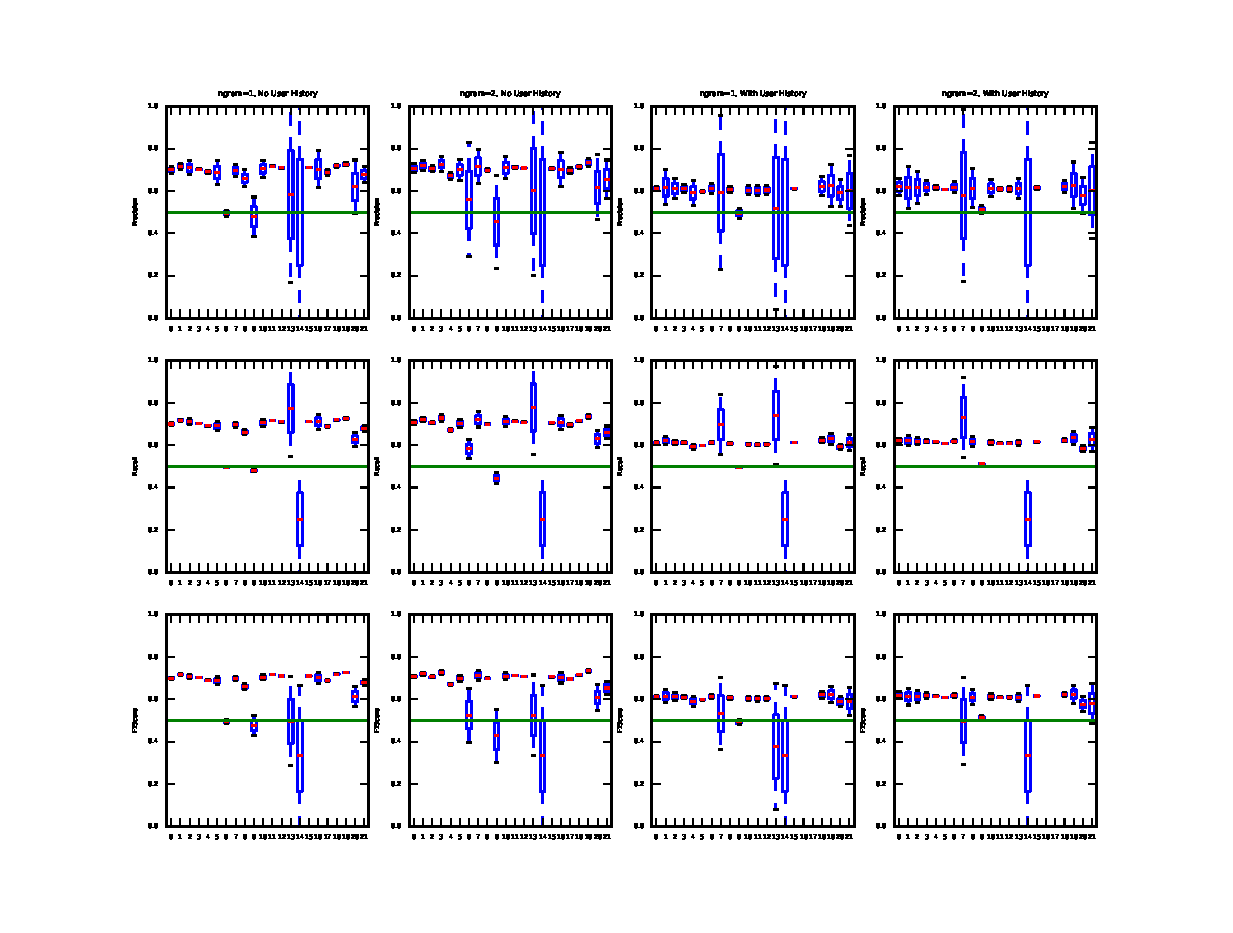
\includegraphics[width=\paperwidth]{figures/binary.eps}
    \caption{Binary classification results}
\end{sidewaysfigure}
\noindent\begin{sidewaysfigure}
    \centering
    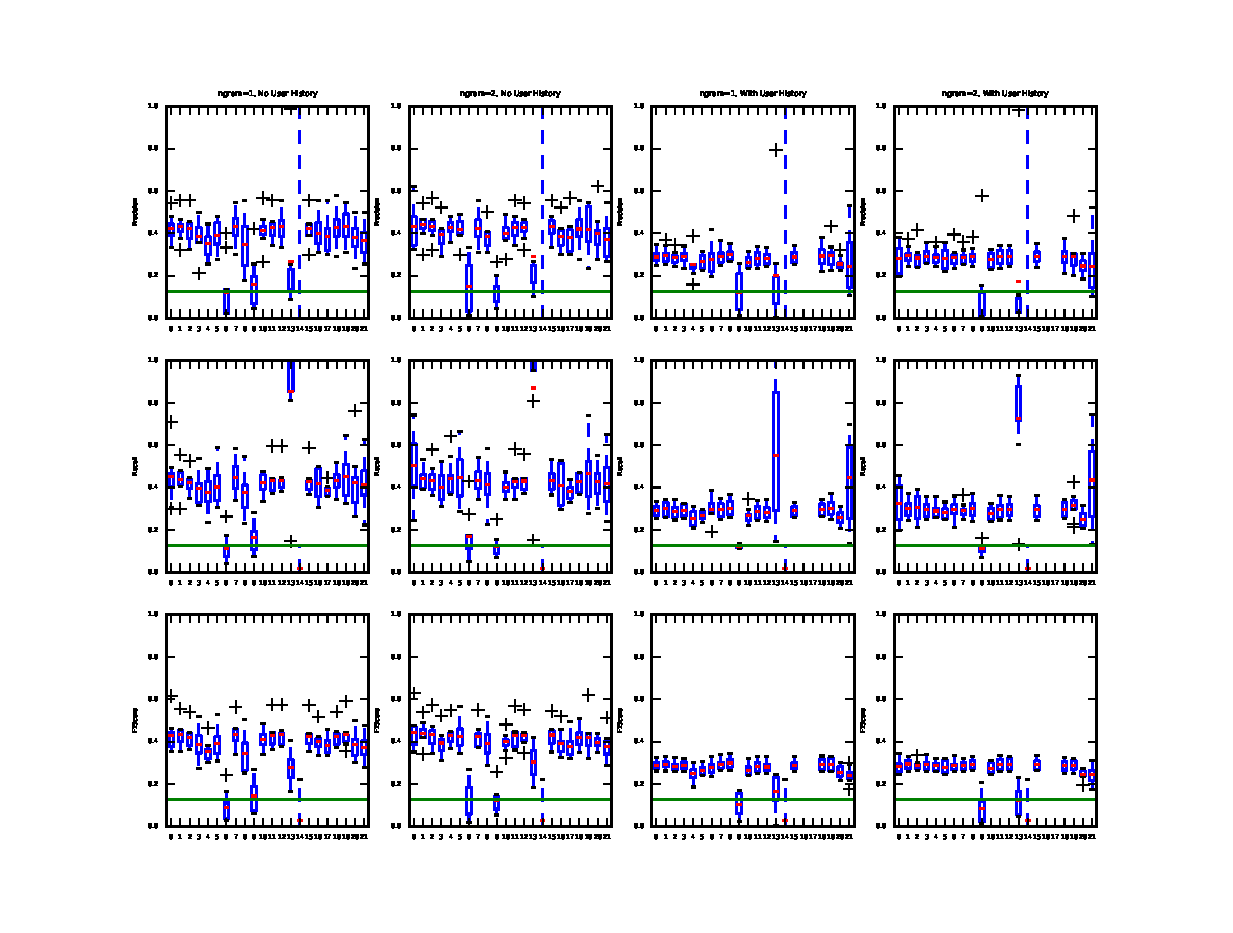
\includegraphics[width=\paperwidth]{figures/multi_class}
    \caption{Multi-Class classification results}
\end{sidewaysfigure}
\newpage

\bibliographystyle{alpha}
\bibliography{paper}
\end{document}
